\chapter{System Hardware Architecture}

First we'll illustrate system's architecture from a global point of view, then we will show more in detail system's hardware and software organization.

\section{Global overview}

System global overview is shown in Figure \ref{fig:sysml}, using SysML diagrams. {\em Block Definition Diagram} highlights separation between software modules and how hardware components are controlled by different software modules, while {\em Internal Block Diagram} is used to show data flows between the various hardware components.

\begin{figure}[tp]
    \centering
    \subfloat[System stereotypes, defined in a SysML profile]{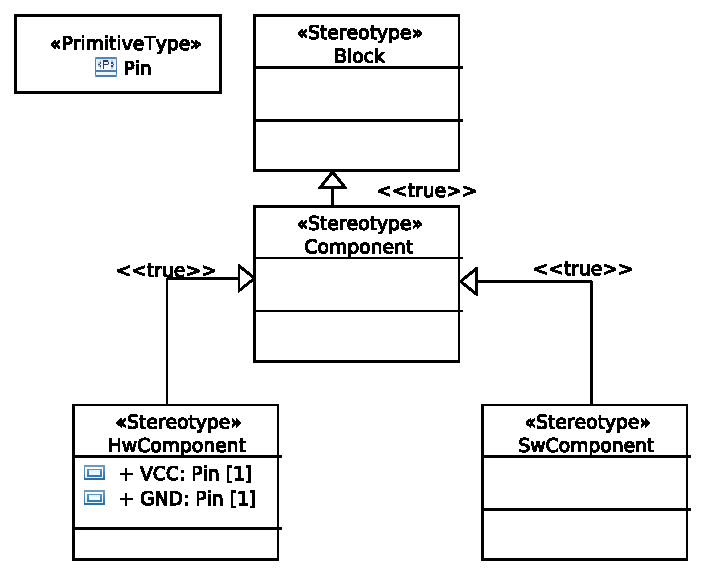
\includegraphics[width=0.6\textwidth, keepaspectratio]{img/StereotypeD}\label{fig:sysml_stereo}}
    ~\\
    \subfloat[System Block Definition Diagram]{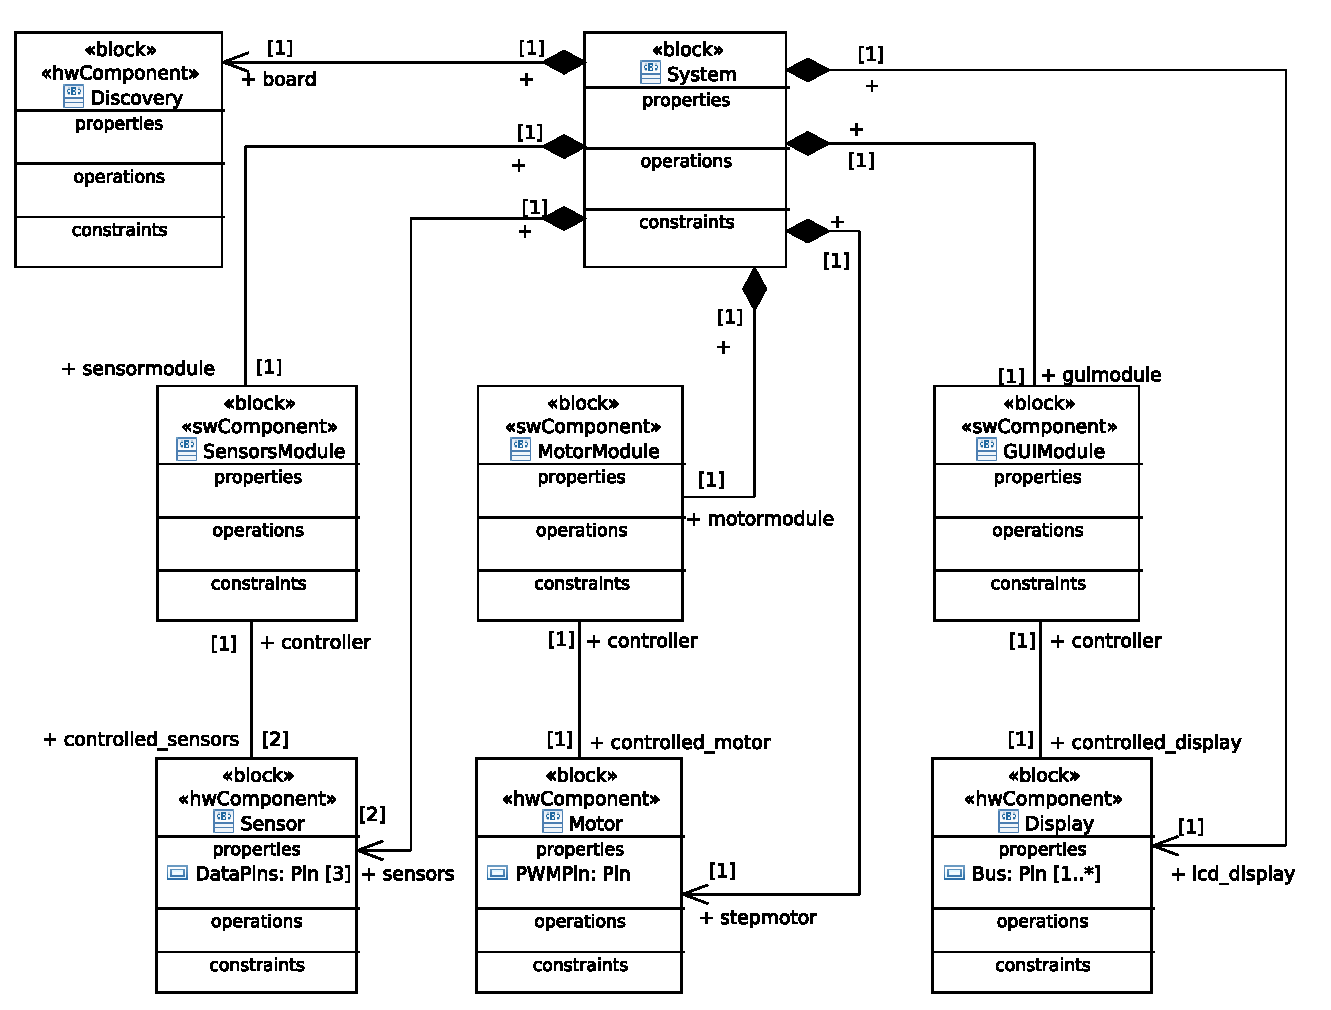
\includegraphics[width=\textwidth, keepaspectratio]{img/BlockDefinitionD}\label{fig:sysml_block}}
    \caption{System architecture shown using SysML diagrams.}\label{fig:sysml}
\end{figure}
\begin{figure}[tp]
    \ContinuedFloat
    \centering
    ~\\
    \subfloat[A bounded feasible region]{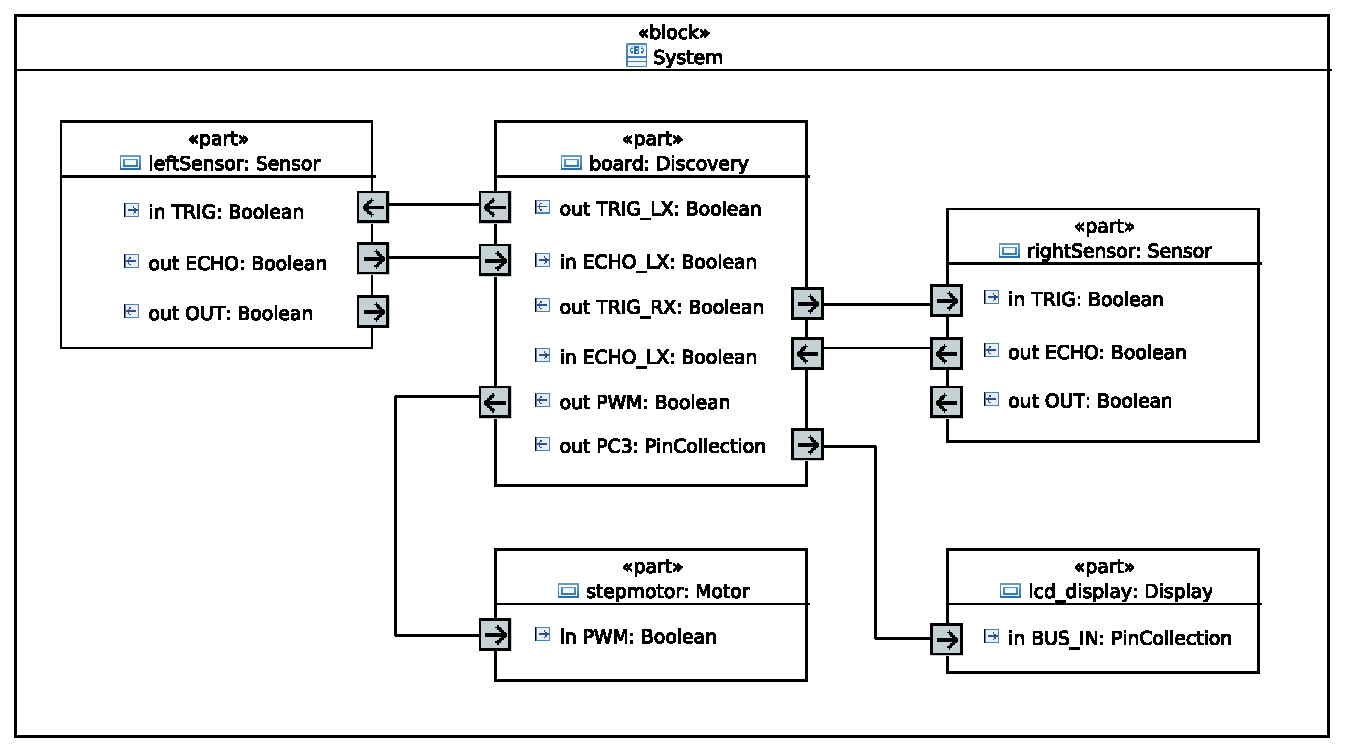
\includegraphics[width=\textwidth, keepaspectratio]{img/InternalBlockD}\label{fig:sysml_internal}}
    \caption{System architecture shown using SysML diagrams. (cont.)}
\end{figure}


\section{Hardware components}

Hardware components choice was driven by parts availability and their price per unit. We will first illustrate external hardware components, before moving on describing briefly the used microcontroller.

\subsection{Ultrasonic sensors}

To detect obstacles in front of the system two two ultrasonic distance sensors have been used. The choice fell on two \textit{HY-SRF05} sensors, shown in Figure \ref{fig:sensor}. Ultrasonic sensors overcome many of the weaknesses of IR sensors, the latter affected easily by color of obstacles and lighting of the environment. On the contrary, ultrasonic sensors provide precise distance measurement regardless of these conditions, because they use ultrasonic sound waves.

%% TODO: crop images
\begin{figure}[htp]
\centering
\hspace*{\fill}
\subfloat[Sensor's appearance]{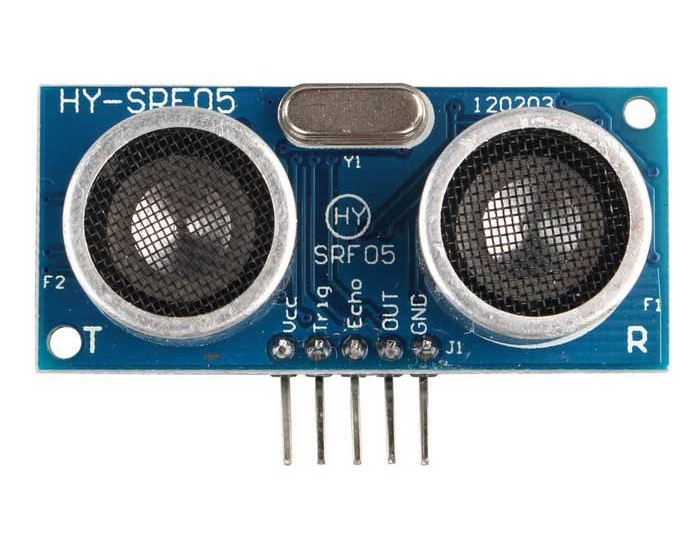
\includegraphics[width=0.4\textwidth,keepaspectratio]{img/hy-srf05.jpg}\label{fig:sensor_appearance}}
\hfill
\subfloat[Sensor's dimension]{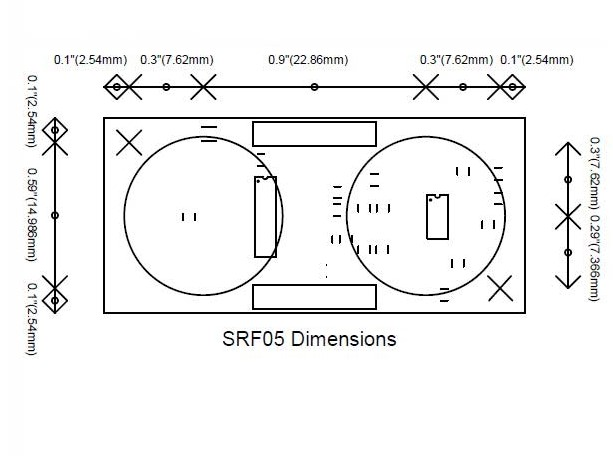
\includegraphics[width=0.5\textwidth,keepaspectratio]{img/hy-srf05-dim.jpg}\label{fig:sensor_dimensions}}
\hspace*{\fill}\\
\caption{HY-SRF05 Ultrasonic Distance Sensor.}
\label{fig:sensor}
\end{figure}

To check if an object is in the area covered by the ultrasonic sensor, it is needed to supply a pulse at least \SI{10}{\micro\second} long to the {\em trigger} input. The HY-SRF05 will send out an 8 cycle burst of ultrasound at \SI{40}{\kilo\hertz} and raise its echo line to high value. It then listens for an echo, and as soon as the sensor detects the echo it will lower down echo line value again.

The echo line is therefore a pulse whose width is exactly the time needed by the ultrasonic wave to hit an obstacle and come back to the sensor. Dividing this time by 2 times the speed of sound will give us the distance of the object. If nothing is detected then the HY-SRF05 will lower its echo line anyway after about \SI{30}{\milli\second}.





\subsection{Servo motor}

In order to change sensors' position a servo motor is used. A typical servo consists of a small electric motor driving a train of reduction gears. In particular for this work, the choice fell on HS-645MG from Hitec, shown in Figure \ref{fig:motor}.

\begin{figure}[tp]
\centering
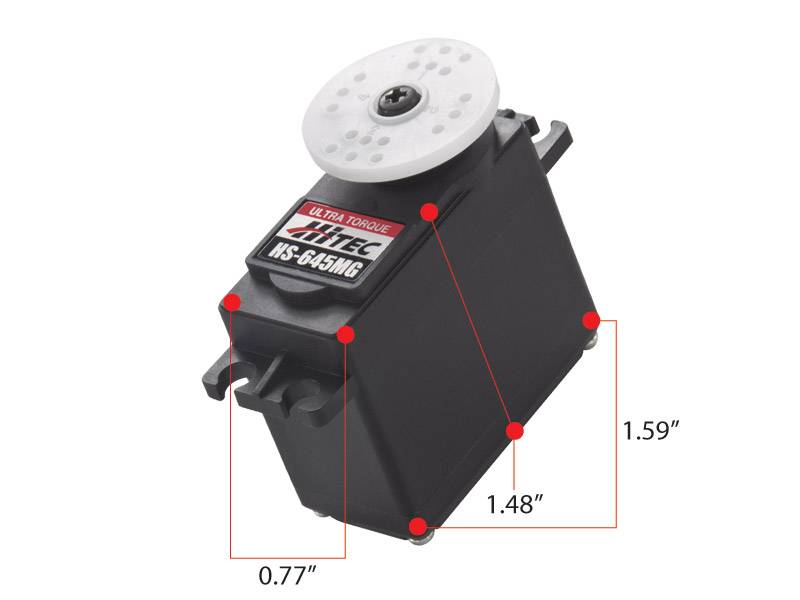
\includegraphics[width=0.6\textwidth,keepaspectratio]{img/hs-645mg.jpg}
\caption{HS-645MG servo motor}
\label{fig:motor}
\end{figure}

The servo motor will constantly check whether the position of the arm is correct with respect to the desired position, expressed as PWM signal, generating a correction torque, either clockwise or counterclockwise, in case we want to move to another position. This way the mechanical arm mounted on top of motor's shaft will move from one desired orientation angle to another.

The PWM signal used to control this servo motor expresses the desired position in terms of duration of the pulse sent at a constant frequency. To keep the motor in the same position, the same pulse must be repeated at the working frequency. Working frequency of a HS-645MG is \SI{50}{\hertz}, while minimum and maximum positions are expressed respectively by sending pulses \si{700} and \SI{2300}{\micro\second} long.


%The position of the output, measured by the potentiometer, is continually compared to the commanded position from the control. Any difference gives rise to an error signal in the appropriate direction, which drives the electric motor either forwards or backwards, and moving the output shaft to the commanded position. This kind of motors are controlled by sending an electrical pulse of variable width (PWM), through the control wire. There is a minimum pulse, a maximum pulse, and a repetition rate. The PWM sent to the motor determines position of the shaft, and based on the duration of the pulse sent via the control wire the rotor will turn to the desired position. Servos will not hold their position forever, hence the position pulse must be repeated to instruct the servo to stay in position. In the HS-645MG the repetition frequency (or working frequency) is $50Hz$ and the minimum - maximum PWM amplitude are respectively $900-2100 \mu s$

\subsection{Development board and LCD}

These devices are controlled by a STM32F4 Discovery board, which runs both controller and applicative code using ERIKA OS as real-time operating system. The Discovery Board is shown in Figure \ref{fig:board_board}. Power can be provided to the board using a standard USB Mini Type-B connector, connected to a \SI{5}{V} power supply\footnote{Power supply must not supply more than \SI{100}{\milli\ampere}.}; board includes also a voltage regulator and two buttons, respectively a reset button and a user button.

%Basically all the computation needed to drive the motor, activate/read the sensors and to display on a LCD screen are executed on a STM32F4 micro controller based on the ARM Cortex-M4F core. In particular, to provide a quick and easy way for engineers to evaluate their micro controller chips, STM built a development board. The one chosen is the STM32F4 Discovery. The power for each board is provided by a choice of the 5 V via the USB cable, or an external 5 V power supply. They can be used as output power supplies of 3 V or 5 V (current must be less than 100 mA). The board also include a voltage regulator, reset button, user button and multiple LEDs. 


\begin{figure}
\centering
\hspace*{\fill}
\subfloat[STM32F4 Discovery board]{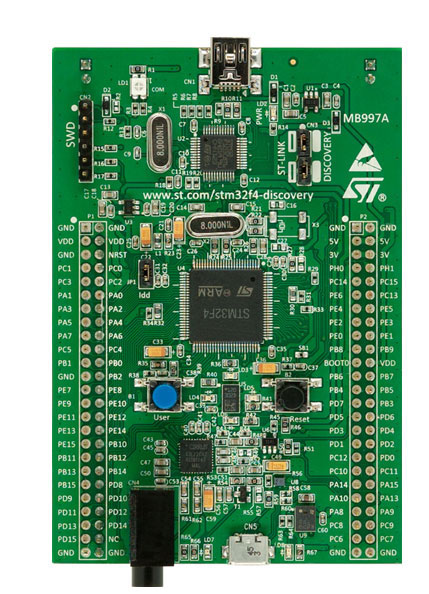
\includegraphics[width=0.34\textwidth,keepaspectratio]{img/stm32f4.jpg}\label{fig:board_board}}
\hfill
\subfloat[Expansion board for STM32F4 Discovery board]{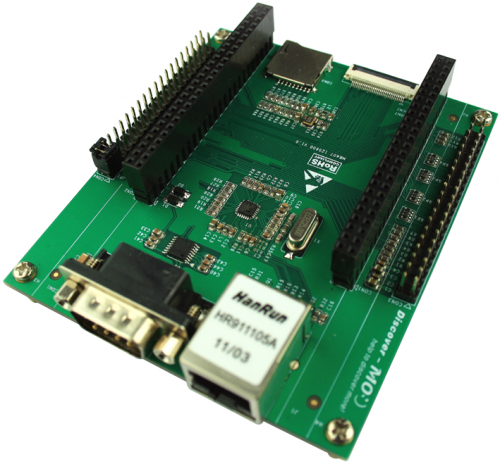
\includegraphics[width=0.34\textwidth,keepaspectratio]{img/baseboard.png}\label{fig:board_expansion}}
\hspace*{\fill}
\\
\subfloat[LCD Screen included with Expansion board kit]{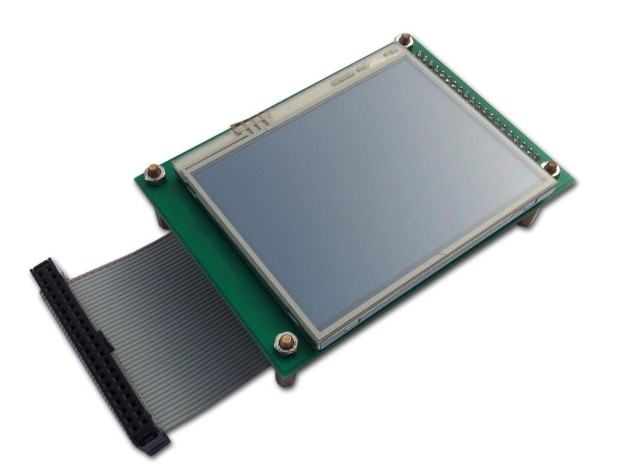
\includegraphics[width=0.6\textwidth,keepaspectratio]{img/lcd.jpg}\label{fig:board_lcd}}

\caption{STM32F4 Discovery kit}
\label{fig:board}
\end{figure}

Since the system requires a screen on which to show detected obstacles' positions, an Expansion kit was needed to connect the Discovery board to his LCD screen (STM32F4DIS-LCD). This kit includes both the LCD screen and an Expansion board (STM32F4DIS-EXT), which expands basic functionalities of the Discovery board providing additional connectors (like Ethernet and serial ones), a MicroSD card slot and connectors for LCD or camera peripherals. Expansion board and its LCD screen are both shown in Figure \ref{fig:board}.


% In order to use the LCD screen (STM32F4DIS-LCD) an expansion board is needed. The expansion board STM32F4DIS-EXT expands the functionality of the STM32F4 Discovery providing a microSD card slot, ethernet connectivity and extension connectors for LCD or camera boards.


\section{Connections and wiring}

External peripherals have been connected to the board using a small circuit obtained from a small perforated board. We will illustrate each peripheral pin and wiring scheme in following sections, while full wiring scheme can be found in Figure \ref{fig:wire_scheme}.

\begin{figure}[htp]
\centering
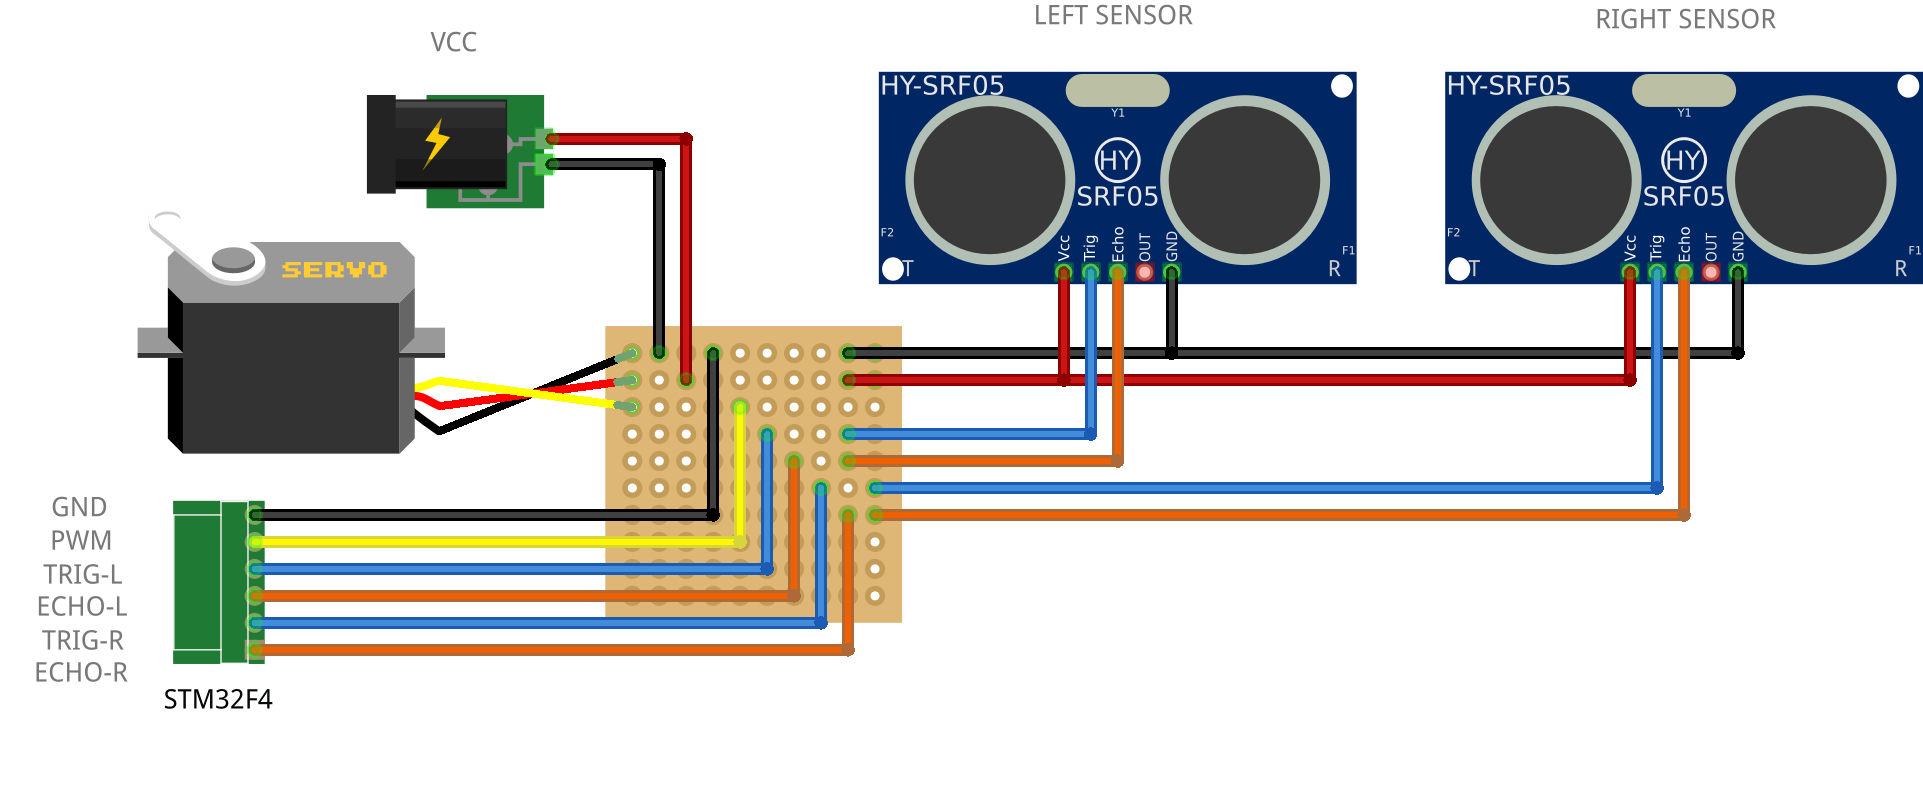
\includegraphics[width=0.8\textwidth, keepaspectratio]{img/wire-schema.png}
\caption{Full wiring scheme between external peripherals and the Discovery board}
\label{fig:wire_scheme}
\end{figure}



\subsection{Servo motor connection}
Hitec servomotors come with a universal connector called ``S'' connector. Meanings of individual wires in this connector are shown in Table \ref{tab:wire_motor}. The Discovery board has been connected to appropriate right connectors adopting the wiring scheme shown in Figure \ref{fig:wire_motor}. The PWM signal has been provided using the port and pin assigned to PWM output, as declared in Table \ref{tab:func_data_dictionary}.

%All of our Hitec servos come with the “S” or universal connector. The yellow cable is used to drive the motor with a PWM signal generated by the STM32F4 discovery board. The red and the black cable are respectively the VCC and the GND of the motor.

\begin{table}[p]
\centering

\begin{tabular}{c|c|c}
\hline
\textbf{Name} & \textbf{Cable color} & \textbf{Description}    \\ \hline
SIGNAL        & Yellow               & PWM signal to the motor \\
VCC           & Red                  & Electricity supply      \\
GND           & Black                & Ground                 
\end{tabular}
\caption{Servo motor ``S'' connector pin meanings}
\label{tab:wire_motor}
\end{table}

\begin{figure}[p]
\centering
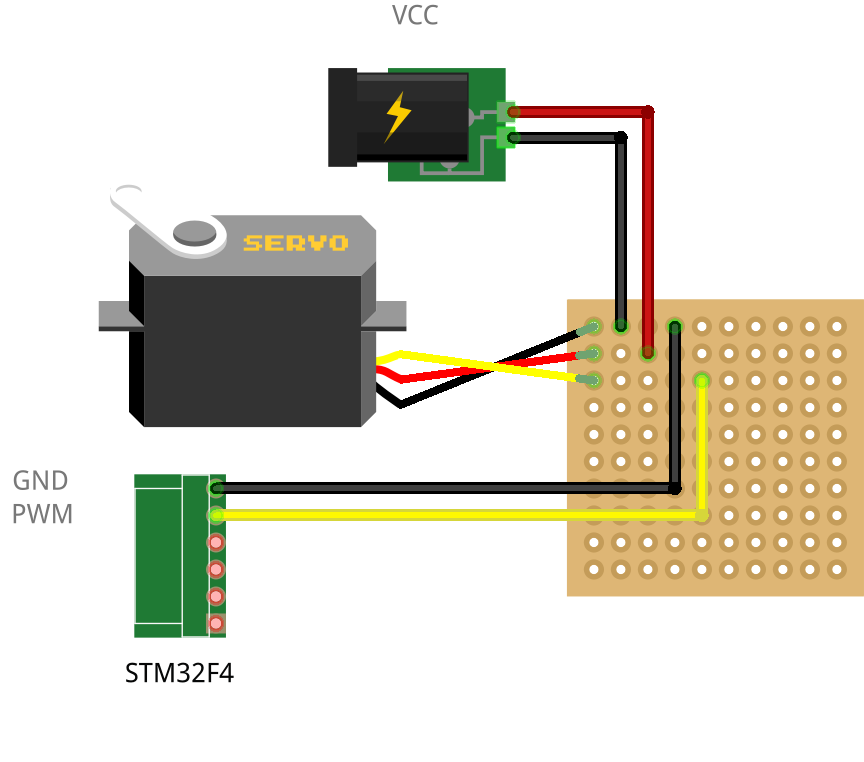
\includegraphics[width=0.7\textwidth,keepaspectratio]{img/wire-servo.png}
\caption{Servo motor wiring scheme}
\label{fig:wire_motor}
\end{figure}




\subsection{Ultrasonic sensors connection}

HY-SRF05 sensors have 5 pins, whose meanings are shown in Table \ref{tab:wire_sensor}. These sensors can be used in two different configurations, wither using one pin both for trigger/echo or 2 separate pins. The 2 pins mode is the default one and can be selected by simply leaving the OUT pin unconnected. The Discovery board has been connected to right pins adopting the wiring scheme shown in Figure \ref{fig:wire_sensor}. Each sensors' pin has been connected to the relative board one, as declared in Table \ref{tab:func_data_dictionary}. 

% Hence, VCC PIN is connected to the electricity supply (5V), the GND PIN is connected to the ground, the OUT PIN is leaved unconnected and the Trig PIN/Echo PIN are connected separately to the board.

\begin{table}[p]
\centering
\begin{tabular}{c|c}
\hline
\textbf{Pin} & \textbf{Description}                         \\ \hline
VCC          & Power supply                                 \\
TRIG         & \SI{10}{\micro\second} pulse trigger input   \\
ECHO         & Sensor response                              \\
OUT          & Change sensor mode                           \\
GND          & Ground                  
\end{tabular}
\caption{Ultrasonic sensors connection}
\label{tab:wire_sensor}
\end{table}

\begin{figure}[p]
\centering
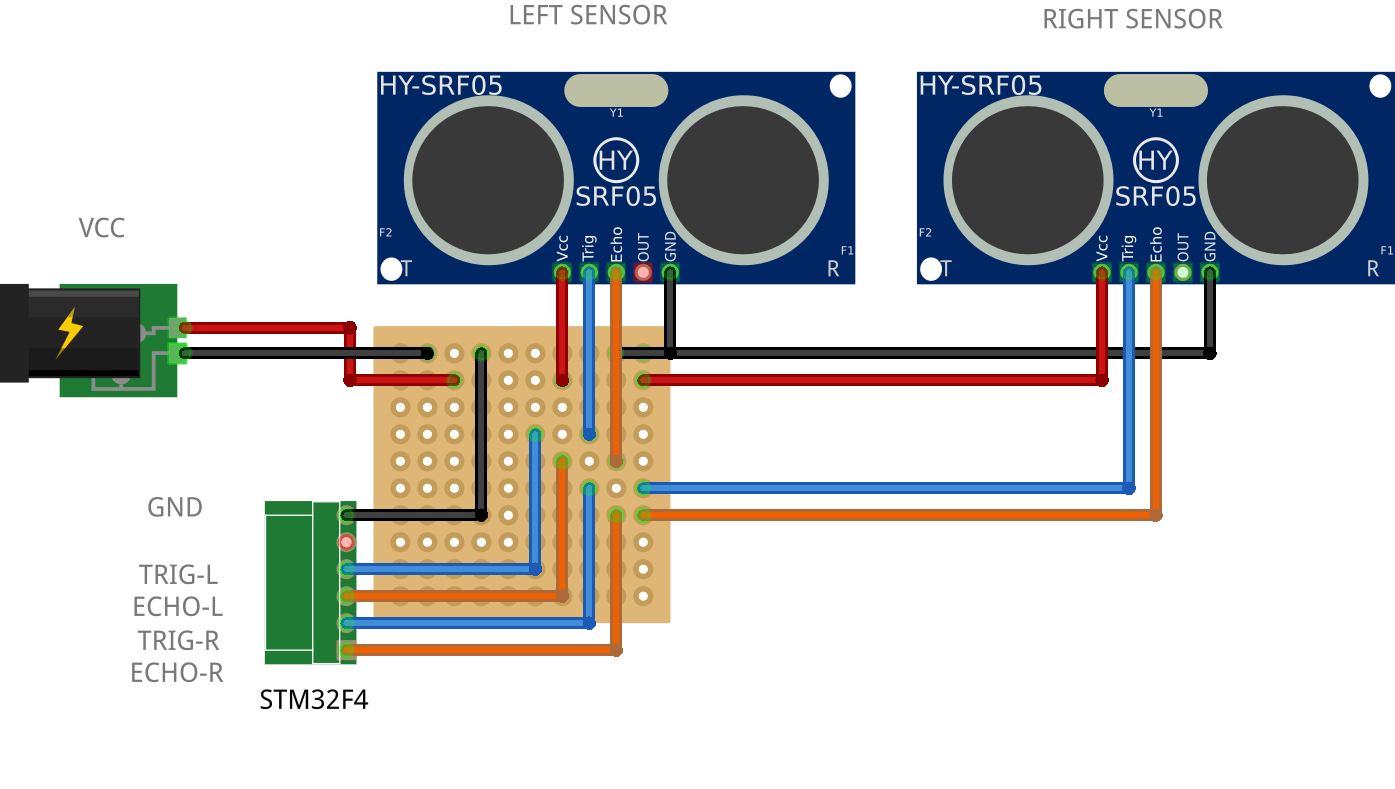
\includegraphics[width=0.8\textwidth, keepaspectratio]{img/wire-sensors.png}
\caption{Ultrasonic sensor wiring scheme}
\label{fig:wire_sensor}
\end{figure}

\begin{figure}[p]
\centering
\includegraphics[width=0.8\textwidth, keepaspectratio]{img/Sonar.png}
\caption{Appearance of the final system.}
\label{fig:sonar}
\end{figure}




